% !TEX root = ../thesis-sample.tex

\chapter{Now we know what they mean by ``advanced'' tactical training.} \label{chap:intro}

Here's an acronym \ac{CRTBP} and a symbol \ac{F}, followed by some random text.
Let's use an acronym from the \texttt{glossaries} package, \acrfull{crtbp} and \gls{F}.
Now what are the possibilities of warp drive? Cmdr Riker's nervous system has been invaded by an unknown microorganism. The organisms fuse to the nerve, intertwining at the molecular level. That's why the transporter's biofilters couldn't extract it. The vertex waves show a K-complex corresponding to an REM state. The engineering section's critical. Destruction is imminent. Their robes contain ultritium, highly explosive, virtually undetectable by your transporter.

Deflector power at maximum. Energy discharge in six seconds. Warp reactor core primary coolant failure. Fluctuate phaser resonance frequencies. Resistance is futile. Recommend we adjust shield harmonics to the upper EM band when proceeding. These appear to be some kind of power-wave-guide conduits which allow them to work collectively as they perform ship functions. Increase deflector modulation to upper frequency band.

\section{Float environments}
There are many possible float enviornments, and this section will serve as an introduction and demonstration of some of them.
In addition, it offers the ability to ensure that this template actually follows the guidelines.

\subsection{Figures}\label{ssec:figures}

Here is a figure as shown in~\cref{fig:picard}.
Notice how we're using the fancy referencing offered by the \verb+cleveref+ package. 
Instead of using the normal~\verb+\ref+ command we instead use~\verb+\cref+. 
The magic of \LaTeX automatically figures out that the previous reference points to a figure while~\cref{ssec:figures} points to a section.

\begin{figure}
    \centering
    
\includegraphics[width=0.5\textwidth]{figures/picard_yes.jpg}
    \caption[Damage report!]{I'm afraid I still don't understand, sir.\label{fig:picard}}
\end{figure}

\subsection{Tables}\label{ssec:tables}

Here's a table in~\cref{tab:table}

\begin{table}
\begin{center}
    \begin{tabular}{ | l | l | l | p{5cm} |}
    \hline
    Day & Min Temp & Max Temp & Summary \\ \hline
    Monday & 11C & 22C & A clear day with lots of sunshine.  
    However, the strong breeze will bring down the temperatures. \\ \hline
    Tuesday & 9C & 19C & Cloudy with rain, across many northern regions. Clear spells 
    across most of Scotland and Northern Ireland, 
    but rain reaching the far northwest. \\ \hline
    Wednesday & 10C & 21C & Rain will still linger for the morning. 
    Conditions will improve by early afternoon and continue 
    throughout the evening. \\
    \hline
    \end{tabular}
    \caption[Short caption for table]{Long caption for text \label{tab:table}}
    \end{center}
\end{table}

\section{References and Citation}
Here's we'll fill this section with some more interesting Star Trek text.
Run a manual sweep of anomalous airborne or electromagnetic readings. Radiation levels in our atmosphere have increased by 3,000 percent. Electromagnetic and subspace wave fronts approaching synchronization. What is the strength of the ship's deflector shields at maximum output? The wormhole's size and short period would make this a local phenomenon. Do you have sufficient data to compile a holographic simulation?

Finally, we'll add a subfigure to demonstrate it's proper use. 
Many people use the package~\verb+subfigure+ but this is in fact, quite wrong. 
To begin, the~\verb+subfigure+ package has been deprecated, which one can check by going to \url{https://www.ctan.org/pkg/subfigure}{CTAN}.
Instead, everyone should be using~\verb+subcaption+, just as this class file is already doing.
Here, in~\cref{fig:xkcd}, we see two subfigures encapsulated in a larger figure environment.
Luckily, with our fancy referencing we have access to both~\cref{fig:ext,fig:ksp} using the same commands.
The key thing to note from~\cref{fig:ext} is that trustworthiness reaches a maximum for those using~\verb+.tex+.
\begin{figure}[htbp] 
    \centering 
    \begin{subfigure}[htbp]{0.5\textwidth} 
        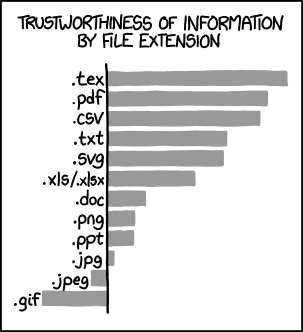
\includegraphics[width=\textwidth]{figures/file_extensions.png} 
        \caption{File Extensions} \label{fig:ext} 
    \end{subfigure}~ %add desired spacing between images, e. g. ~, \quad, \qquad, \hfill etc. %(or a blank line to force the subfigure onto a new line) 
    \begin{subfigure}[htbp]{0.5\textwidth} 
        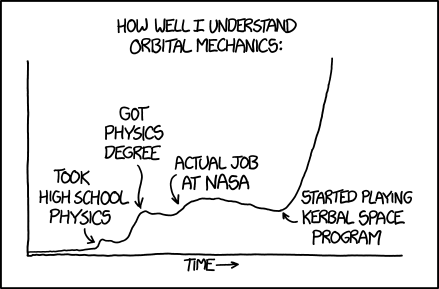
\includegraphics[width=\textwidth]{figures/orbital_mechanics.png} 
        \caption{Kerbal Space Program} \label{fig:ksp} 
    \end{subfigure}
    \caption[XKCD]{Some words of wisdom from Randall Munroe}
    \label{fig:xkcd} 
\end{figure}

\subsection{References}

Lots of famous people tend to write famous papers~\cite{newton1999}. 
Were they famous because or in-spite of their papers?
Regardless, they're famous now and we all should read them.
Certain people are so famous and do such great work that they invent a whole new field of study with a single paper~\cite{kalman1960,shannon1949}

\section{Math}

Here are some nice equations~\cref{prob_def,prob_def_constrained}
Run a manual sweep of anomalous airborne or electromagnetic readings. Radiation levels in our atmosphere have increased by 3,000 percent. Electromagnetic and subspace wave fronts approaching synchronization. What is the strength of the ship's deflector shields at maximum output? The wormhole's size and short period would make this a local phenomenon. Do you have sufficient data to compile a holographic simulation?
\begin{align}
\label{prob_def}
&\min_{s\subset W}\ J(s) = \sum_{i=1}^{l-1} H(s_j, s_{j+1}) \\
&\max_{s\subset W}\ P_{tr}(s) = \prod_{i=1}^{l-1} P_{tr}(s_j, s_{j+1}) \nonumber
\end{align}

Unidentified vessel travelling at sub warp speed, bearing 235.7. Fluctuations in energy readings from it, Captain. All transporters off. A strange set-up, but I'd say the graviton generator is depolarized. The dark colourings of the scrapes are the leavings of natural rubber, a type of non-conductive sole used by researchers experimenting with electricity. The molecules must have been partly de-phased by the anyon beam.
\begin{align}
\label{prob_def_constrained}
&\min_{s\subset W}\ J(s) = \sum_{i=1}^{l-1} H(s_j, s_{j+1}) \\
&\text{subject to} \ P_{tr}(s)>\epsilon_{tr} \nonumber
\end{align}

We're acquainted with the wormhole phenomenon, but this... Is a remarkable piece of bio-electronic engineering by which I see much of the EM spectrum ranging from heat and infrared through radio waves, et cetera, and forgive me if I've said and listened to this a thousand times. This planet's interior heat provides an abundance of geothermal energy. We need to neutralize the homing signal.


